%-----------------------------------------------------------------------------%
\chapter{\babTiga}
\label{bab:3}
%-----------------------------------------------------------------------------%

Bab ini membahas tentang metodologi penelitian yang dilakukan dalam penelitian ini. Metodologi penelitian ini mencakup langkah penelitian, skenario dan metrik evaluasi dari penelitian yang dilakukan.


%-----------------------------------------------------------------------------%
\section{Langkah Penelitian}
\label{sec:langkahPenelitian}
%-----------------------------------------------------------------------------%

Penelitian dilakukan dengan lima tahap seperti yang terdapat pada 
\pic~\ref{fig:metode}. Tahap tersebut mencakup rumusan masalah, studi literatur, perancangan arsitektur, \textit{smart contract} dan simulator, evaluasi, dan penarikan kesimpulan.

\begin{figure}
	\centering
	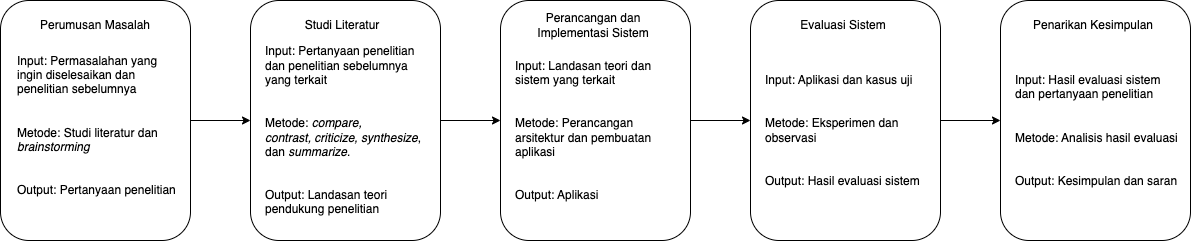
\includegraphics[width=\textwidth]{assets/pics/metode}
	\caption{Langkah penelitian.}
	\label{fig:metode}
\end{figure}

Tahapan pertama dalam penelitian ini adalah perumusan masalah. Penulis merumuskan masalah yang berasal dari permasalahan proses \textit{delivery order} pada sistem INSW saat ini dan literatur-literatur terkait. Kemudian dipilih satu masalah yang disorot untuk kemudian dioptimisasi. Perumusan masalah ini menghasilkan pertanyaan penelitian.

Tahapan kedua adalah studi literatur. Penulis melakukan pencarian atas penelitian terkait dengan pertanyaan penelitian. Penulis melakukan \textit{compare, contrast, criticize, synthesize, dan summarize} atas literatur-literatur terkait sehingga membentuk suatu landasan teori yang dapat menjadi pendukung penelitian. 

Tahapan ketiga adalah perancangan arsitektur, \textit{smart contract}, dan simulator. Dilakukan perancangan \textit{logic} \textit{smart contract} menggunakan Hyperledger Fabric SDK untuk proses bisnis pembuatan permohonan \textit{delivery order}. Pada tahap ini juga dirancang arsitektur untuk kebutuhan \textit{testing} atau simulasi. Kemudian dirancang simulator untuk dilakukan simulasi dan eksperimen terhadap \textit{smart contract} yang telah dibuat.

Kemudian, untuk tahapan keempat adalah evaluasi sistem. Dilakukan pengujian \textit{smart contract} dengan simulator yang telah dibuat. Hasil simulasi dan eksperimen kemudian dianalisis dan dievaluasi.

Terakhir, tahapan kelima pada penelitian ini ditarik sebuah kesimpulan dari hasil analisis dan evaluasi eksperimen. Tahapan ini menghasilkan jawaban dari pertanyaan-pertanyaan penelitian yang dirumuskan pada tahap pertama serta saran untuk penelitian selanjutnya.


\section{Metrik Evaluasi}
\label{sec:metrikevaluasi}

Pada penelitian ini, dilakukan uji dan evaluasi \textit{smart contract} menggunakan simulator yang dibuat. Skenario simulasi didasarkan pada permasalahan-permasalahan pada sistem INSW saat ini. Metode evaluasi berupa analisis \textit{log} aplikasi. Evaluasi pertama berupa analisis keamanan berdasarkan aspek fungsionalitas, \textit{authentication}, \textit{access control}, \textit{failure rate}, dan \textit{availability}.

Evaluasi fungsionalitas berkaitan dengan pengujian fitur \textit{delivery order} dalam sistem berbasis \textit{blockchain} dengan Hyperledger Fabric. Evaluasi dilakukan dengan melakukan pemanggilan pada \textit{smart contract} melalui simulator. Hasil evaluasi berupa analisis deskriptif dari log yang diambil dari log \textit{peer} dan log \textit{smart contract}. Aspek ini bertujuan untuk mengetahui apakah fitur \textit{delivery order} dapat diimplementasikan menggunakan Hyperledger Fabric.

Evaluasi selanjutnya adalah aspek \textit{authentication}. Pengujian dilakukan dengan melakukan pengaksesan sistem \textit{blockchain} menggunakan \textit{credential} atau identitas yang tidak terdaftar atau tidak diberikan \textit{permission} untuk mengakses \textit{blockchain}. Aspek ini bertujuan untuk mengetahui jika hanya pihak yang terdaftar atau memiliki izin yang dapat mengakses \textit{blockchain}.

Aspek ketiga yang dievaluasi adalah \textit{access control}. Pengujian ini ditujukan untuk pembatasan operasi tertentu pada \textit{smart contract} untuk dapat dilakukan hanya oleh pihak yang terotorisasi. Pengujian dilakukan dengan melakukan operasi terbatas dengan identitas yang tidak berwenang melakukan operasi tersebut.

Selanjutnya untuk melakukan evaluasi \textit{failure rate} dan \textit{availability}, sistem diuji dengan melakukan simulasi pembuatan \textit{delivery order} dalam waktu yang bersamaan dengan jumlah yang inkremental. Kemudian dilakukan analisis terhadap perubahan-perubahan yang terjadi saat jumlah \textit{request} ditingkatkan. Pengujian ini dilakukan untuk mengukur kapasitas sistem saat beban tinggi.
